\section{Siamese networks}
\label{siamese networks}

Section~\ref{acrhitecture} describes our overall network architecture for entity matching. Section~\ref{loss_functions} enumerates the different loss functions which have been used in prior work, and a new loss function which appears to do better in metric learning for entities.  Section~\ref{triplet_selection} describes a novel triplet selection mechanisms for entity matching.

\subsection{Network Architecture}
\label{architecture}
\begin{figure}
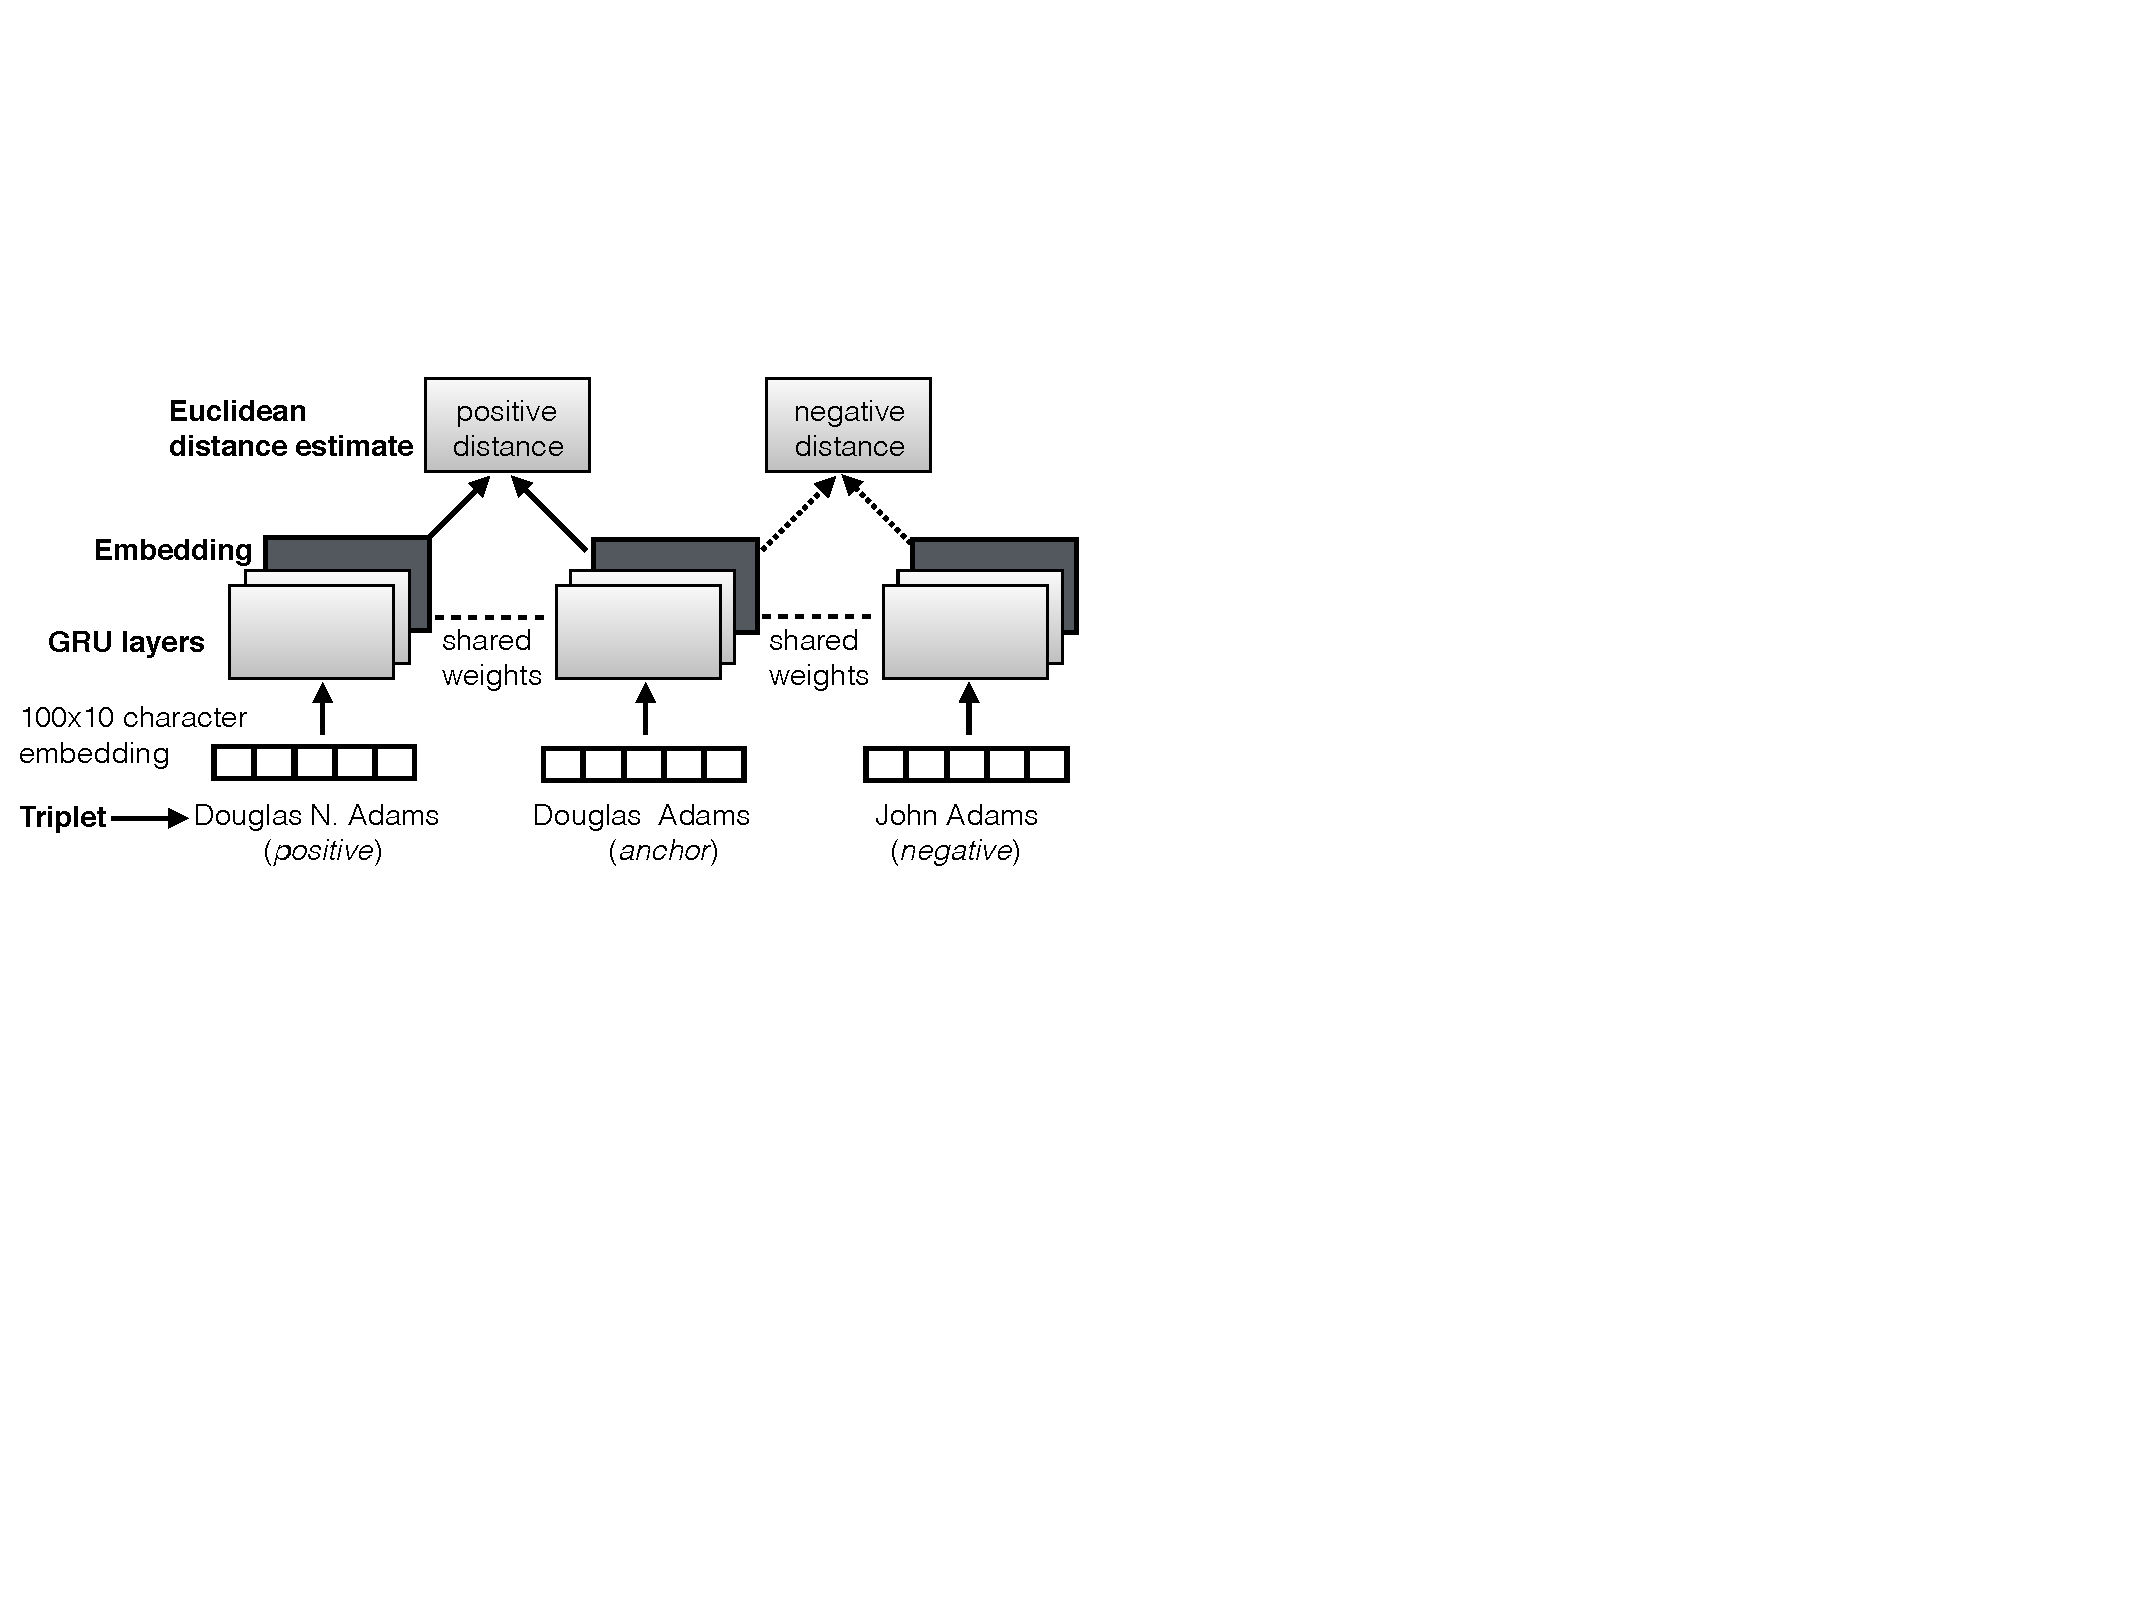
\includegraphics[width=1.0\linewidth]{triplet_siamese_network}
\caption{Architecture of the siamese network}
\label{siamese_nets}
\end{figure}

Figure~\ref{siamese_nets} illustrates overall network architecture we used to build a system for fuzzy joins.  Input vectors were computed assuming a maximum name length of 10 for each entity (i.e., no entity could have a name that spanned more than 10 words).  A 100 dimensional character embedding was computed for each `word' in the entity using pretrained embeddings \cite{hashimoto-jmt:2017:EMNLP2017}, which resulted in a 100 x 10 character encoding for each name used in a triplet.  As described earlier, in a triplet, each entity name (or \textit{anchor}) is paired with another name for the same entity (or \textit{positive}), and with a name for a completely different entity (or \textit{negative}).  The three input vectors from each triplet are fed to three identical networks that share the same weights.  Weight sharing ensures that the networks learn the same mapping function for any given input vector.  In our implementation, each of the three networks had 4 stacked layers of 128 unit Gated Recurrent Units (or GRUs) to capture the sequential nature of the input.  

GRUs are a type of recurrent network \cite{cho-al-emnlp14} where each hidden unit updates its weights at a specific step in the sequence $t$ based on the current input $x_t$ and the value of the hidden unit from the prior step $h_{t-1}$.  $r_t$ is a reset gate which determines whether the state from the previous step $h_{t-1}$ should be ignored. $z_t$ is an update gate which determines whether the current hidden state should be updated with the new hidden state $\tilde{h_t}$.  Equations~\ref{eq_1}-\ref{eq_4} that govern the update at $h_t$, as summarized by \cite{colah}.
\begin{equation}
z_t = \sigma(W_z . [h_{t-1}, x_t])
\label{eq_1}
\end{equation}

\begin{equation}
r_t = \sigma(W_r . [h_{t-1}, x_t])
\label{eq_2}
\end{equation}

\begin{equation}
\tilde{h_t} = tanh (W . [r_t * h_{t-1}, x_t])
\label{eq_3}
\end{equation}

\begin{equation}
h_t = (1- z_t) * h_{t-1} + z_t * \tilde{h_t}
\label{eq_4}
\end{equation}

The output of the last layer shown in the Figure~\ref{siamese_nets} as a dark gray layer produces a vector embedding for the inputs.  These are fed to two layers which compute a euclidean distance between the \textit{anchor} and the \textit{positive} elements of a triplet (\textit{positive distance}), and the \textit{anchor} and the \textit{negative} elements of a triplet (\textit{negative distance}).  Conceptually, there are two dual objects in metric learning, one to minimize \textit{positive distances}, and the other to maximize \textit{negative distances}.  As described below, this dual objective is achieved by different loss functions in the literature.

\subsection{Loss functions}
\label{loss_functions}
Let $f(x)$ represent an embedding for an entity name, $f(x_i^a)$,$f(x_i^p)$, $f(x_i^n)$ reflect the vector embeddings of the \textit{anchor}, \textit{positive} and \textit{negative}, respectively.  We investigated four different loss functions to explore their effectiveness for the entity metric learning problem.
\begin{itemize}
\item For face recognition, Schroff et al. \cite{DBLP:conf/cvpr/SchroffKP15} propose a triplet loss function where the squared \textit{positive distances} for each triplet $i$ in the set of $N$ triplets is separated from the squared \textit{negative distances} by a margin of $\alpha$:
\begin{equation}
  L = \sum_{i}^N(\left[\|f(x_i^a) - f(x_i^p)\|_{2}^2 - \|f(x_i^a)- f(x_i^n)\|_{2}^2 + \alpha \right]
\label{schroff}
\end{equation}
Note that in this formulation, it is assumed that embedding is normalized so $\| f(x) \|_2 = 1$.  In other words, the vector embeddings are normalized using the L2 norm.  The value of $\alpha$ in the original work \cite{DBLP:conf/cvpr/SchroffKP15} is also set to 0.2.
\end{itemize}
